\documentclass[10pt, french]{article}
%% -----------------------------
%% Préambule
%% -----------------------------
% !TEX encoding = UTF-8 Unicode
% LaTeX Preamble for all cheatsheets
% Author : Gabriel Crépeault-Cauchon

% HOW-TO : copy-paste this file in the same directory as your .tex file, and add in your preamble the next command right after you have specified your documentclass : 
% \input{preamble-cheatsht.tex}
% ---------------------------------------------
% ---------------------------------------------

% Extra note : this preamble creates document that are meant to be used inside the multicols environment. See the documentation on internet for further information.

%% -----------------------------
%% Encoding packages
%% -----------------------------
\usepackage[utf8]{inputenc}
\usepackage[T1]{fontenc}
\usepackage{babel}
\usepackage{lmodern}

%% -----------------------------
%% Variable definition
%% -----------------------------
\def\auteur{Gabriel Crépeault-Cauchon / Nicholas Langevin}
\def\BackgroundColor{white}

%% -----------------------------
%% Margin and layout
%% -----------------------------
% Determine the margin for cheatsheet
\usepackage[landscape, hmargin=1cm, vmargin=1.7cm]{geometry}
\usepackage{multicol}

% Remove automatic indentation after section/subsection title.
\setlength{\parindent}{0cm}

% Save space in cheatsheet by removing space between align environment and normal text.
\usepackage{etoolbox}
\newcommand{\zerodisplayskips}{%
  \setlength{\abovedisplayskip}{0pt}%
  \setlength{\belowdisplayskip}{0pt}%
  \setlength{\abovedisplayshortskip}{0pt}%
  \setlength{\belowdisplayshortskip}{0pt}}
\appto{\normalsize}{\zerodisplayskips}
\appto{\small}{\zerodisplayskips}
\appto{\footnotesize}{\zerodisplayskips}

%% -----------------------------
%% URL and links
%% -----------------------------
\usepackage{hyperref}
\hypersetup{colorlinks = true, urlcolor = gray!70!white, linkcolor = black}

%% -----------------------------
%% Document policy (uncomment only one)
%% -----------------------------
%	\usepackage{concrete}
	\usepackage{mathpazo}
%	\usepackage{frcursive} %% permet d'écrire en lettres attachées
%	\usepackage{aeguill}
%	\usepackage{mathptmx}
%	\usepackage{fourier} 

%% -----------------------------
%% Math configuration
%% -----------------------------
\usepackage[fleqn]{amsmath}
\usepackage{amsthm,amssymb,latexsym,amsfonts}
\usepackage{empheq}
\usepackage{numprint}
\usepackage{dsfont} % Pour avoir le symbole du domaine Z

% Mathematics shortcuts

\newcommand{\reels}{\mathbb{R}}
\newcommand{\entiers}{\mathbb{Z}}
\newcommand{\naturels}{\mathbb{N}}
\newcommand{\eval}{\biggr \rvert}
\usepackage{cancel}
\newcommand{\derivee}[1]{\frac{\partial}{\partial #1}}
\newcommand{\prob}[1]{\Pr \left( #1 \right)}
\newcommand{\esp}[1]{\mathrm{E} \left[ #1 \right]} % espérance
\newcommand{\variance}[1]{\mathrm{Var} \left( #1   \right)}
\newcommand{\covar}[1]{\mathrm{Cov} \left( #1   \right)}
\newcommand{\laplace}{\mathcal{L}}
\newcommand{\deriv}[2][]{\frac{\partial^{#1}}{\partial #2^{#1}}}
\newcommand{\e}[1]{\mathrm{e}^{#1}}
\newcommand{\te}[1]{\text{exp}\left\{#1\right\}}
\DeclareMathSymbol{\shortminus}{\mathbin}{AMSa}{"39}



% To indicate equation number on a specific line in align environment
\newcommand\numberthis{\addtocounter{equation}{1}\tag{\theequation}}

%
% Actuarial notation packages
%
\usepackage{actuarialsymbol}
\usepackage{actuarialangle}

%
% Matrix notation for math symbols (\bm{•})
%
\usepackage{bm}
% Matrix notation variable (bold style)
\newcommand{\matr}[1]{\mathbf{#1}}



%% -----------------------------
%% tcolorbox configuration
%% -----------------------------
\usepackage[most]{tcolorbox}
\tcbuselibrary{xparse}
\tcbuselibrary{breakable}

%%
%% Coloured box "definition" for definitions
%%
\DeclareTColorBox{definition}{ o }				% #1 parameter
{
	colframe=blue!60!green,colback=blue!5!white, % color of the box
	breakable, 
	pad at break* = 0mm, 						% to split the box
	title = {#1},
	after title = {\large \hfill \faBook},
}
%%
%% Coloured box "definition2" for definitions
%%
\DeclareTColorBox{definitionNOHFILL}{ o }				% #1 parameter
{
	colframe=blue!60!green,colback=blue!5!white, % color of the box
	pad at break* = 0mm, 						% to split the box
	title = {#1},
	before title = {\faBook \quad },
	breakable
}


%%
%% Coloured box "algo" for algorithms
%%
\newtcolorbox{algo}[ 1 ]
{
	colback = blue!5!white,
	colframe = blue!75!black,
	title=#1,
	fonttitle = \bfseries,
	breakable
}
%%
%% Coloured box "conceptgen" for points adding to a concept's deifintion
%%
\newtcolorbox{conceptgen}[ 1 ]
{
	breakable,
	colback = beaublue,
	colframe = airforceblue,
	title=#1,
	fonttitle = \bfseries
}
%%
%% Coloured box "probch3" pour formules relatives au 3ème chapitre de prob
%%
\newtcolorbox{probch3}[ 1 ]
{
	colback = ruddypink,
	colframe = burgundy,
	fonttitle = \bfseries,	
	breakable,
	title=#1
}
%%
%% Coloured box "formula" for formulas
%%
\newtcolorbox{formula}[ 1 ]
{
	colback = green!5!white,
	colframe = green!70!black,
	breakable,
	fonttitle = \bfseries,
	title=#1
}
%%
%% Coloured box "formula" for formulas
%%
\DeclareTColorBox{algo2}{ o }
{
	enhanced,
	title = #1,
	colback=blue!5!white,	
	colbacktitle=blue!75!black,
	fonttitle = \bfseries,
	breakable,
	boxed title style={size=small,colframe=arsenic} ,
	attach boxed title to top center = {yshift=-3mm,yshifttext=-1mm},
}
%%
%% Coloured box "examplebox" for formulas
%%
\newtcolorbox{examplebox}[ 1 ]
{
	colback = lightmauve,
	colframe = antiquefuchsia,
	breakable,
	fonttitle = \bfseries,title=#1
}
%%
%% Coloured box "rappel" pour rappel de formules
%%
\newtcolorbox{rappel}[ 1 ]
{
	colback = ashgrey,
	colframe = arsenic,
	breakable,
	fonttitle = \bfseries,title=#1
}
%%
%% Coloured box "rappel" pour rappel de formules
%%
\DeclareTColorBox{rappel_enhanced}{ o }
{
	enhanced,
	title = #1,
	colback=ashgrey, % color of the box
%	colframe=blue(pigment),
%	colframe=arsenic,	
	colbacktitle=arsenic,
	fonttitle = \bfseries,
	breakable,
	boxed title style={size=small,colframe=arsenic} ,
	attach boxed title to top center = {yshift=-3mm,yshifttext=-1mm},
}
%%
%% Coloured box "notation" for notation and terminology
%%
\DeclareTColorBox{distributions}{ o }			% #1 parameter
{
	enhanced,
	title = #1,
	colback=gray(x11gray), % color of the box
%	colframe=blue(pigment),
	colframe=arsenic,	
	colbacktitle=aurometalsaurus,
	fonttitle = \bfseries,
	boxed title style={size=small,colframe=arsenic} ,
	attach boxed title to top center = {yshift=-3mm,yshifttext=-1mm},
	breakable
%	left=0pt,
%  	right=0pt,
%    box align=center,
%    ams align*
%  	top=-10pt
}

%% -----------------------------
%% Graphics and pictures
%% -----------------------------
\usepackage{graphicx}
\usepackage{pict2e}
\usepackage{tikz}

%% -----------------------------
%% insert pdf pages into document
%% -----------------------------
\usepackage{pdfpages}

%% -----------------------------
%% Color configuration
%% -----------------------------
\usepackage{color, soulutf8, colortbl}


%
%	Colour definitions
%
\definecolor{blue(munsell)}{rgb}{0.0, 0.5, 0.69}
\definecolor{blue(matcha)}{rgb}{0.596, 0.819, 1.00}
\definecolor{blue(munsell)-light}{rgb}{0.5, 0.8, 0.9}
\definecolor{bleudefrance}{rgb}{0.19, 0.55, 0.91}
\definecolor{blizzardblue}{rgb}{0.67, 0.9, 0.93}
\definecolor{bondiblue}{rgb}{0.0, 0.58, 0.71}
\definecolor{blue(pigment)}{rgb}{0.2, 0.2, 0.6}
\definecolor{bluebell}{rgb}{0.64, 0.64, 0.82}
\definecolor{airforceblue}{rgb}{0.36, 0.54, 0.66}
\definecolor{beaublue}{rgb}{0.74, 0.83, 0.9}
\definecolor{cobalt}{rgb}{0.0, 0.28, 0.67}	% nice light blue-ish
\definecolor{blue_rectangle}{RGB}{83, 84, 244}		% ACT-2004
\definecolor{indigo(web)}{rgb}{0.29, 0.0, 0.51}	% purple-ish
\definecolor{antiquefuchsia}{rgb}{0.57, 0.36, 0.51}	%	pastel dark purple ish
\definecolor{darkpastelpurple}{rgb}{0.59, 0.44, 0.84}
\definecolor{gray(x11gray)}{rgb}{0.75, 0.75, 0.75}
\definecolor{aurometalsaurus}{rgb}{0.43, 0.5, 0.5}
\definecolor{ruddypink}{rgb}{0.88, 0.56, 0.59}
\definecolor{pastelred}{rgb}{1.0, 0.41, 0.38}		
\definecolor{lightmauve}{rgb}{0.86, 0.82, 1.0}
\definecolor{azure(colorwheel)}{rgb}{0.0, 0.5, 1.0}
\definecolor{darkgreen}{rgb}{0.0, 0.2, 0.13}			
\definecolor{burntorange}{rgb}{0.8, 0.33, 0.0}		
\definecolor{burntsienna}{rgb}{0.91, 0.45, 0.32}		
\definecolor{ao(english)}{rgb}{0.0, 0.5, 0.0}		% ACT-2003
\definecolor{amber(sae/ece)}{rgb}{1.0, 0.49, 0.0} 	% ACT-2004
\definecolor{green_rectangle}{RGB}{131, 176, 84}		% ACT-2004
\definecolor{red_rectangle}{RGB}{241,112,113}		% ACT-2004
\definecolor{amethyst}{rgb}{0.6, 0.4, 0.8}
\definecolor{amethyst-light}{rgb}{0.6, 0.4, 0.8}
\definecolor{ashgrey}{rgb}{0.7, 0.75, 0.71}			% dark grey-black-ish
\definecolor{arsenic}{rgb}{0.23, 0.27, 0.29}			% light green-beige-ish gray
\definecolor{amaranth}{rgb}{0.9, 0.17, 0.31}
\definecolor{brickred}{rgb}{0.8, 0.25, 0.33}
\definecolor{pastelred}{rgb}{1.0, 0.41, 0.38}

%
% Useful shortcuts for coloured text
%
\newcommand{\orange}{\textcolor{orange}}
\newcommand{\red}{\textcolor{red}}
\newcommand{\cyan}{\textcolor{cyan}}
\newcommand{\blue}{\textcolor{blue}}
\newcommand{\green}{\textcolor{green}}
\newcommand{\purple}{\textcolor{magenta}}
\newcommand{\yellow}{\textcolor{yellow}}

%% -----------------------------
%% Enumerate environment configuration
%% -----------------------------
%
% Custum enumerate & itemize Package
%
\usepackage{enumitem}
%
% French Setup for itemize function
%
\frenchbsetup{StandardItemLabels=true}
%
% Change default label for itemize
%
\renewcommand{\labelitemi}{\faAngleRight}


%% -----------------------------
%% Tabular column type configuration
%% -----------------------------
\newcolumntype{C}{>{$}c<{$}} % math-mode version of "l" column type
\newcolumntype{L}{>{$}l<{$}} % math-mode version of "l" column type
\newcolumntype{R}{>{$}r<{$}} % math-mode version of "l" column type
\newcolumntype{f}{>{\columncolor{green!20!white}}p{1cm}}
\newcolumntype{g}{>{\columncolor{green!40!white}}m{1.2cm}}
\newcolumntype{a}{>{\columncolor{red!20!white}$}p{2cm}<{$}}	% ACT-2005
% configuration to force a line break within a single cell
\usepackage{makecell}


%% -----------------------------
%% Fontawesome for special symbols
%% -----------------------------
\usepackage{fontawesome}

%% -----------------------------
%% Section Font customization
%% -----------------------------
\usepackage{sectsty}
\sectionfont{\color{\SectionColor}}
\subsectionfont{\color{\SubSectionColor}}

%% -----------------------------
%% Footer/Header Customization
%% -----------------------------
\usepackage{lastpage}
\usepackage{fancyhdr}
\pagestyle{fancy}

%
% Header
%
\fancyhead{} 	% Reset
\fancyhead[L]{Aide-mémoire pour~ \cours ~(\textbf{\sigle})}
\fancyhead[R]{\auteur}

%
% Footer
%
\fancyfoot{}		% Reset
\fancyfoot[R]{\thepage ~de~ \pageref{LastPage}}
\fancyfoot[L]{\href{https://github.com/ressources-act/Guide_de_survie_en_actuariat}{\faGithub \ ressources-act/Guide de survie en actuariat}}
%
% Page background color
%
\pagecolor{\BackgroundColor}




%% END OF PREAMBLE
% ---------------------------------------------
% ---------------------------------------------
%% -----------------------------
%% Redefine from template
%% -----------------------------
\def\auteur{Alec James van Rassel et Olivier Côté}
%% -----------------------------
%% Variable definition
%% -----------------------------
\def\cours{Analyse et traitement collectif du risque}
\def\sigle{ACT-1005}
%% -----------------------------
%% Colour setup for sections
%% -----------------------------
\def\SectionColor{brickred}
\def\SubSectionColor{amaranth}
\def\SubSubSection{pastelred}
%%	pour timeline
\usetikzlibrary{shapes,positioning}
\newcommand{\foo}{\hspace{-2.3pt}$\bullet$ \hspace{5pt}}
\usepackage{booktabs}
\usepackage{tabularx}


%\setcounter{section}{1}

%% -----------------------------
%% Début du document
%% -----------------------------
\begin{document}

\begin{multicols*}{3} 
\section{Le risque et l'assurance}
\begin{definitionNOHFILL}[Risque]
\begin{description}
	\item[\textbf{Un} risque:] Un événement dont l'occurrence est (habituellement) aléatoire pouvant causer un dommage à des personnes et/ou des biens;
	\item[\textbf{Le} risque:] La probabilité de survenance de l'événement et l'ampleur de ses conséquences;
\end{description}

Il y \textbf{deux composantes} aux risques:
\begin{itemize}
	\item	La \textbf{probabilité d'occurrence} d'un événement accidentel;
	\item	La \textbf{gravité} des effets (ou conséquences) \textit{financière} de l'événement;
\end{itemize}

Donc du point de vue d'un assureur, le risque est l'\textbf{exposition} à un \textit{événement} dommageable inhérent à une situation (ou activité). 

Quelques \textbf{exemples} d'événements dont l'exposition peut être prise en charge par une compagnie:
\begin{itemize}
	\item	Une compagnie d'assurance auto assure une personne contre le risque d'un accident automobile;
	\item	Une compagnie d'assurance de voyage assure une personne contre le \textbf{danger} (toujours sous forme de conséquence \textit{financière}, que ce soit au niveau de la responsibilité civile, des frais médicaux etc.) d'aller au Mexique;
%%%	-----
%%%	NOTE:
%%%	+	Danger de se faire voler? Tuer? Je ne suis pas certain;
%%% + J'ai émis mon hypothèse, à revoir avec Isabelle ~ OC ~
%%%	-----
\end{itemize}
\end{definitionNOHFILL}

\begin{definitionNOHFILL}[Aversion]
L'aversion au risque est la \textit{peur} d'un investisseur d'un risque qu'il juge trop important.
(L'antonyme de l'\textit{aversion} au risque serait la \textit{tolérance} de celui-ci)

L'aversion au risque se caractérise par une personne qui:
\begin{itemize}
	\item	Ne souhaite pas courir le risque et va vouloir le \textbf{transférer};
	\item[]	Pour exemple, assurer sa maison contre le risque d'inondation;
	\item	Ne juge pas d'être en mesure de supporter le risque et \textbf{refuse} de s'y exposer;
	\item[]	Pour exemple, ne pas faire de parachutisme;
\end{itemize}
	
Le \textbf{degré d'aversion} au risque est \textbf{variable} selon l'intervenant (tous on une aversion au risque, seul le \textit{degré d'aversion} diffère). Par exemple, même les compagnies d'assurance se \textit{\textbf{ré}}assurent. 

Habituellement, elles ont moins d'aversion au risque qu'un individu en raison de leur:
\begin{itemize}
	\item	\textbf{capacité financière};
	\item	La \textbf{mise en commun} des risques;
\end{itemize} 

Lorsqu'un individu souhaite \textit{transférer} son risque, il échange au preneur de risque une \textbf{prime de risque}. En assurance, c'est donc une \textit{prime d'assurance} qu'un \textbf{assuré} va payer à sa \textbf{compagnie d'assurance}.
\end{definitionNOHFILL}

\begin{algo}{Gérer du risque}
Différentes \textbf{méthodes} existent pour gérer un risque, pour exemple:
\begin{itemize}[leftmargin = *]
	\item	Évitement (Ex : Éviter d'avoir une voiture);
	\item	Prévention (Conserver le risque réduit grâce à la prévention);
	\item	Prise de risque (\textbf{rétention}) (intentionnelle ou non);
	\item	Transfert (Principe fondamental de l'assurance);
	\item	Diversification des risques (Ne pas tous mettre ces oeufs dans le même panier);
	\item	\textcolor{amaranth}{Couverture des risques (\textbf{hedging}) (Non-Couvert dans le cadre du cours)};
	\item	\textcolor{amaranth}{La titrisation (Non-Couvert dans le cadre du cours)};
\end{itemize}
%
Face à un risque, différents \textbf{comportements} peuvent survenir selon:
\begin{itemize}
	\item	La \textit{perception} du risque;
	\item	L'\textit{aversion} au risque;
	\item	La disponibilité d'\textit{outils} pour gérer des risques;
%%%	-----
%%%	NOTE:
%%%	+	Outils c'est vague, trouver un exemple plus concret;
%%%	+	Genre "outils" dans le sens d'argent ou outils dans le sens de marteaux, etc.?
%%%	+	Je ne suis pas certain de comprendre ce qu'on veut dire;
%%%	-----
\end{itemize}
\end{algo}

\begin{definitionNOHFILL}[L'assurance]
L'assurance est un \textit{système} qui permet de \textit{protéger} un assuré (individu, association, entreprise) contre les \textbf{conséquences \textbf{financières}} découlant de la survenance d'un risque \textit{spécifique}.
%%%	-----
%%%	NOTE:
%%%	+	Je dis "un risque spécifique" au lieu "d'un risque particulier" pour éviter toute confusion avec l'assurance de particuliers / personnes
%%%
%%%	-----

Les assureurs est en mesure de protéger les individus contre un risque grâce à \textit{loi des grands nombres}:
\begin{itemize}
	\item	On associe un assuré à une \textbf{communauté} de personnes---l'ensemble des assurés;
	\item	On \textbf{rassemble} \textit{(pool)} les primes; 
\end{itemize}
Lorsque des risques se réalisent, on \textbf{indemnise} les membres ayant subi des dommages. Ce faisant, la communauté prend \textbf{matériellement} en charge les dommages de ses membres.

On définit donc l'assurance comme un système de gestion des risques basé sur la notion de \textit{solidarité}. Ce \textbf{mécanisme} de l'assurance :
\begin{itemize}
	\item	Ne modifie ni la \textit{fréquence} du risque ni sa \textit{sévérité};
	\item	\textit{Transfère} le risque d'un assuré à un, ou plusieurs, autres;
	\item	\textit{Protège} un assuré contre le risque de survenance d'événements qu'il ne peut pas supporter seul;
	\item	\textit{Permet} à un assuré de réaliser des activités comportant des risques qu'il n'aurait pas autrement pu supporter;
\end{itemize}

Lorsque des risques se réalisent, on \textbf{indemnise} les membres ayant subi des dommages. Ce faisant, la communauté prend \textbf{matériellement} en charge les dommages de ses membres.

\end{definitionNOHFILL}

\begin{algo}{\textbf{Revenu} de l'assureur}
\begin{itemize}
	\item	L'assureur reçoit les \textbf{primes} d'assurance;
	\item	L'assureur \textbf{place l'argent} des assurés, excédentaire des paiements qu'il doit faire, en bourse;
\end{itemize}
Ainsi, il obtient une deuxième source de revenus (primordiale dans le cas d'assurances d'une potentielle longue durée, comme l'\textit{assurance vie}).
\end{algo}


\begin{conceptgen}{Types d'Assurances}
\textbf{1. Assurance de personnes}  

Exemples : 
%\begin{multicols*}{2}
\begin{itemize}[leftmargin = *]
	\item	Décès et longévité;
	\item	Invalidité;
	\item	Perte d'emploi;
	\item	Autres soins de santé (médical et paramédical, dentaire, lunettes);
\end{itemize}  

Certains de ces \textit{risques} sont couverts par l'État, alors que les autres pourront l'être par des compagnies privées.   
%\end{multicols*}

\textbf{2. Assurance IARD} (\textbf{I}ncendie, \textbf{A}ccidents et \textbf{R}isques \textbf{D}ivers)  \textcolor{amaranth}{(Couvert dans le cours \textit{Introduction à l'actuariat I})}  

Exemples pour les \textcolor{amethyst}{individus} et \textcolor{amaranth}{entreprises}:
\begin{itemize}[leftmargin = *]
	\item	\textcolor{amethyst}{Biens (auto, habitation)};
	\item	\textcolor{amaranth}{Biens (auto, bâtiment)};
	\item	\textcolor{amaranth}{Opérations};
\end{itemize}
\end{conceptgen}


\section{La sécurité sociale}

%%%	dans le coin des lignes 520 j'explique comment les tableaux fonctionnent en LaTeX;

\begin{definition}[La sécurité sociale]
\textbf{Programmes} visant à apporter une certaine \textbf{sécurité} afin de ne pas perdre son \textbf{statut} dans la société. Elles visent à \textit{maintenir}, \textit{protéger} et \textit{améliorer} les conditions de vie essentielles.

\begin{itemize}
	\item	Cette \og \textit{assurance} \fg{} est accordée par le gouvernement;
	\item	C'est les \textit{obligations} du gouvernement pour donner un niveau de vie minimum à tous;
\end{itemize}
\end{definition}


\begin{definition}[Organisation internationale du travail (OIT)]
But est de rassembler ses états membres en vue d'une action commune pour:
\begin{itemize}
	\item	\textit{Promouvoir} les \textbf{droits au travail};
	\item	\textit{Encourager} la \textbf{création d'emplois} décents;
	\item	\textit{Développer} la \textbf{protection sociale};
	\item	\textit{Renforcer} le \textbf{dialogue social} dans le domaine du travail;
	\item[]	C'est-à-dire, toutes formes de négociation, consultation, ou d'échange d'information entre gouvernements, employeurs et travailleurs.
\end{itemize}

L'OIT est une:
\begin{itemize}
	\item	Agence spécialisée de l'ONU fondée en 1919 (donc sous l'ancêtre de l'ONU) à Genève;
	\item	Institution tripartite: rassemble les gouvernements, employeurs et travailleurs membres de l'ONU;
\end{itemize}

Pour exemple dans le cadre de sa mission, l'OIT cherche à s'assurer que les enfants ne travaillent pas, qu'il y a égalité homme-femme, etc.
\end{definition}

\begin{conceptgen}{2 conceptions différentes de la sécurité sociale}
\begin{center}
\textbf{Bismark}
\end{center}
\begin{itemize}[leftmargin = *]
	\item	Principe d'\textbf{assurance sociale} lié au \textbf{travail};
	\item	Logique \textbf{assurantielle}
	\item[]	C'est-à-dire que les prestations sont versées aux \textbf{individus assurés} contre tel risque;
	\item	\textbf{Principes} de la protection:
		\begin{enumerate}
		\item	Limité aux travailleurs;
		\item	Protection obligatoire;
			\begin{itemize}
			\item	Pour ceux n'ayant pas assez d'argent pour se couvrir eux-mêmes;
			\end{itemize}
		\item	\textbf{Proportionnalité} des \textbf{cotisations} et \textbf{prestations} au salaire;
			\begin{itemize}
			\item	Pour exemple, le paiement (cotisation) d'assurance chômage qui varie en fonction du salaire;
			\item	Si j'ai un plus grand salaire, ma participation au régime (cotisations) sera plus élevée;
%%%	-----
%%%	NOTE:
%%%	+	Peux-tu vérifier que ce que j'ai écris ci-dessus est cohérent stp? (AJVR)
%%%	-----
			\end{itemize}
			\item	Protection gérée par les salariés et les employeurs;
		\end{enumerate}
	\item	Ce fut la base pour les autres systèmes.
\end{itemize}
\tcbline

\begin{center}
\textbf{Beveridge}
\end{center}
\begin{itemize}[leftmargin = *]
	\item	Principe de protection généralisée, la \textbf{sécurité sociale}, \textbf{sans lien au travail} fondée sur la solidarité;
	\item	Logique \textbf{assistancielle}
	\item[]	C'est-à-dire que les prestations sont versées aux \textbf{individus en besoin};
		\begin{itemize}
		\item	Est-ce qu'une personne a besoin d'un revenu? Si oui, on va l'aider.
		\end{itemize}
	\item	Exemple: chômage
	\item	Principes de protection:
		\begin{enumerate}
		\item	\textbf{Universalité} de la protection sociale;
			\begin{itemize}
			\item	Couverture de toute la population et de tous les risques sociaux;
			\end{itemize}
		\item	\textbf{Uniformité} des prestations;
			\begin{itemize}
			\item	Couverture fondée sur les \textit{besoins} et \textbf{non} les \textit{revenus};
			\end{itemize}
		\item	\textbf{Unicité};
			\begin{itemize}
			\item	Gestion par l'état de tous les programmes;
			\end{itemize}	
		\item	Financement par \textbf{l'impôt};
			\begin{itemize}
			\item	Ce faisant, il est également appelé le système \og nationalww \fg{} 
			\end{itemize}
		\end{enumerate}
\end{itemize}
\end{conceptgen}

\begin{rappel_enhanced}[Déclaration universelle des droits de l'homme (1948)]
\begin{distributions}[Article 22]
Toute personne, en tant que membre de la société, a droit à la sécurité sociale.
\end{distributions}
\begin{distributions}[Article 25]
\begin{enumerate}[leftmargin = *]
	\item	Toute personne a droit à un niveau de vie suffisant pour assurer sa santé, son bien-être et ceux de sa famille.
	\item	La maternité et l'enfance ont droit à une aide et à une assistance spéciale.
\end{enumerate}
\end{distributions}
\end{rappel_enhanced}

\begin{conceptgen}{Fonctions des états membres}
Selon l'OIT, les états membres doivent mettre en place au moins 3 des fonctions suivantes (dont au moins une de 3, 4, 5 et 9): 
\begin{enumerate}[leftmargin = *]
	\item	Soins médicaux;
	\item	Indemnités de maladie: prestations fournies pour rétablir ou améliorer la santé d'une personne;
	\item	Chômage: prestations fournies à une personne ayant perdu son emploi;
	\item	Vieillesse: prestations fournies aux personnes ayant pris leurs retraites selon certaines conditions (âge de la retraite atteint, résidence/nationalité);
	\item	Accident du travail et maladies professionnelles;
	\item	Familles: prestations fournies afin de payer le coûts et satisfaire les besoins d'éducation des enfants et aux personnes à charge;
	\item	Invalidité;
	\item	Maternité;
	\item	Survivants;
\end{enumerate}

Auxquels on peut ajouter:
\begin{multicols*}{3}
\begin{enumerate}[leftmargin = *]
	\item	Logement: prestations fournies (sous condition de ressources) pour aider directement un \textit{ménage} (pas un particulier) à payer le coût de son logement;
	\item	Éducation;
%%%	-----
%%%	NOTE:
%%%	+	Faut trouver une façon de mieux distinguer éducation de famille hmmm;
%%%	-----
	\item	Assistance sociale: pour exemple, les food stamps aux É.-U.;
\end{enumerate}
\end{multicols*}
\end{conceptgen}

\textbf{Événements marquants historiques}
%%%	NOTE: le timeline est splitté en 3 pour qu'il ait sur des différents pages
\newcounter{year}

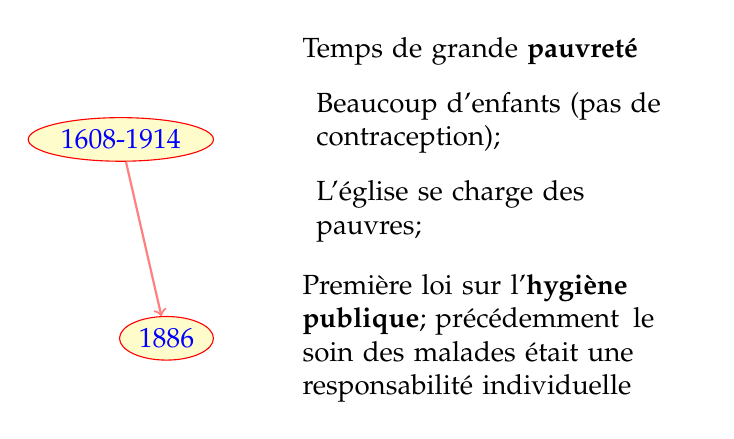
\begin{tikzpicture}[yscale = 0.5,%
           year/.style = {draw	= red,%
           				 text 	= blue,%
           				 fill 	= yellow!20,%
           				 shape 	= ellipse,%
           				 inner sep = 2pt%
           				 },%
           description/.style = {rectangle,%
           				 		align		= left,%
           				 		text width	= 50mm,%
           				 		anchor		= west%
           				 		},%
           timeline/.style = {->,%
           				 	 thick,%
           				 	 red!50%
           				 	 }%
           			]
    \foreach \year/\desc [count=\y] in {%
       1608-1914	/	Temps de grande \textbf{pauvreté}
       	\begin{itemize}[leftmargin = *]
      		\item	Beaucoup d'enfants (pas de contraception);
      		\item	L'église se charge des pauvres;
      	\end{itemize},%
      	1886	/	Première loi sur l'\textbf{hygiène publique}; précédemment\, le soin des malades était une responsabilité individuelle%
       } { \ifnum\y=1 \node[description](\y){\desc};
           \else\node[description,below=1ex of \z](\y){\desc};
           \fi
           \node[year](y-\y) [left=of \y] {\year};
           \ifnum\y>1\draw[timeline] (y-\z)-- (y-\y);\fi
           \global\let\z=\y% for drawing from last node
       }
\end{tikzpicture}
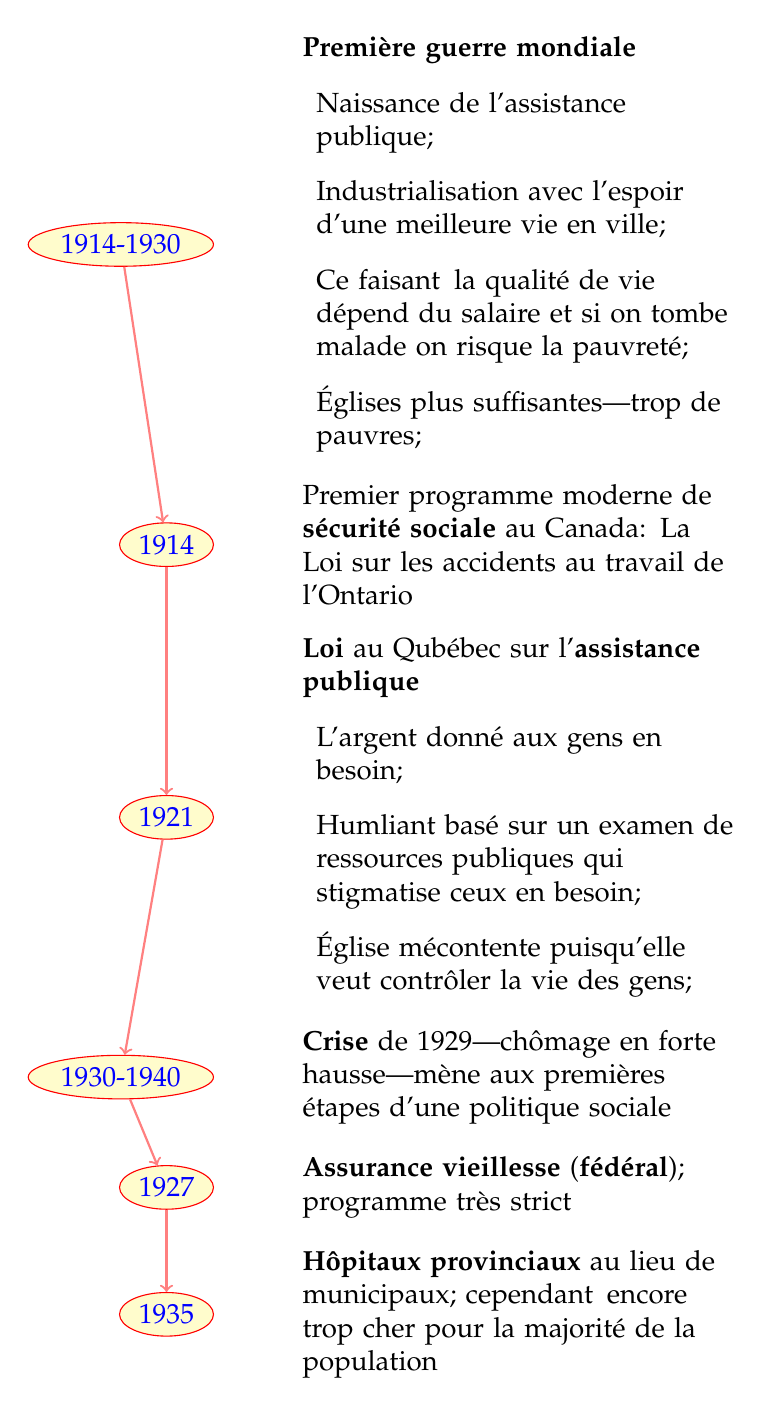
\begin{tikzpicture}[yscale = 0.5,%
           year/.style = {draw	= red,%
           				 text 	= blue,%
           				 fill 	= yellow!20,%
           				 shape 	= ellipse,%
           				 inner sep = 2pt%
           				 },%
           description/.style = {rectangle,%
           				 		align		= left,%
           				 		text width	= 55mm,%
           				 		anchor		= west%
           				 		},%
           timeline/.style = {->,%
           				 	 thick,%
           				 	 red!50%
           				 	 }%
           			]

    \foreach \year/\desc [count=\y] in {%
       1914-1930	/	\textbf{Première guerre mondiale}
       	\begin{itemize}[leftmargin = *]
	       	\item	Naissance de l'assistance publique;
	       	\item	Industrialisation avec l'espoir d'une meilleure vie en ville;
	       	\item[]	Ce faisant\, la qualité de vie dépend du salaire et si on tombe malade on risque la pauvreté;
	       	\item	Églises plus suffisantes---trop de pauvres;
       	\end{itemize}
       ,%
       	1914	/	Premier programme moderne de \textbf{sécurité sociale} au Canada: La Loi sur les accidents au travail de l'Ontario,%
       	1921	/	\textbf{Loi} au Qubébec sur l'\textbf{assistance publique} 
       	\begin{itemize}[leftmargin = *]
       		\item	L'argent donné aux gens en besoin;
      	 	\item	Humliant basé sur un examen de ressources publiques qui stigmatise ceux en besoin;
     	  	\item	Église mécontente puisqu'elle veut contrôler la vie des gens;
       	\end{itemize},%
       1930-1940	/ \textbf{Crise} de 1929---chômage en forte hausse---mène aux premières étapes d'une politique sociale,%
       	1927	/	\textbf{Assurance vieillesse} (\textbf{fédéral}); programme très strict,%
       	1935/	\textbf{Hôpitaux provinciaux} au lieu de municipaux; cependant\, encore trop cher pour la majorité de la population%
       } { \ifnum\y=1 \node[description](\y){\desc};
           \else\node[description,below=1ex of \z](\y){\desc};
           \fi
           \node[year](y-\y) [left=of \y] {\year};
           \ifnum\y>1\draw[timeline] (y-\z)-- (y-\y);\fi
           \global\let\z=\y% for drawing from last node
       }

\end{tikzpicture}
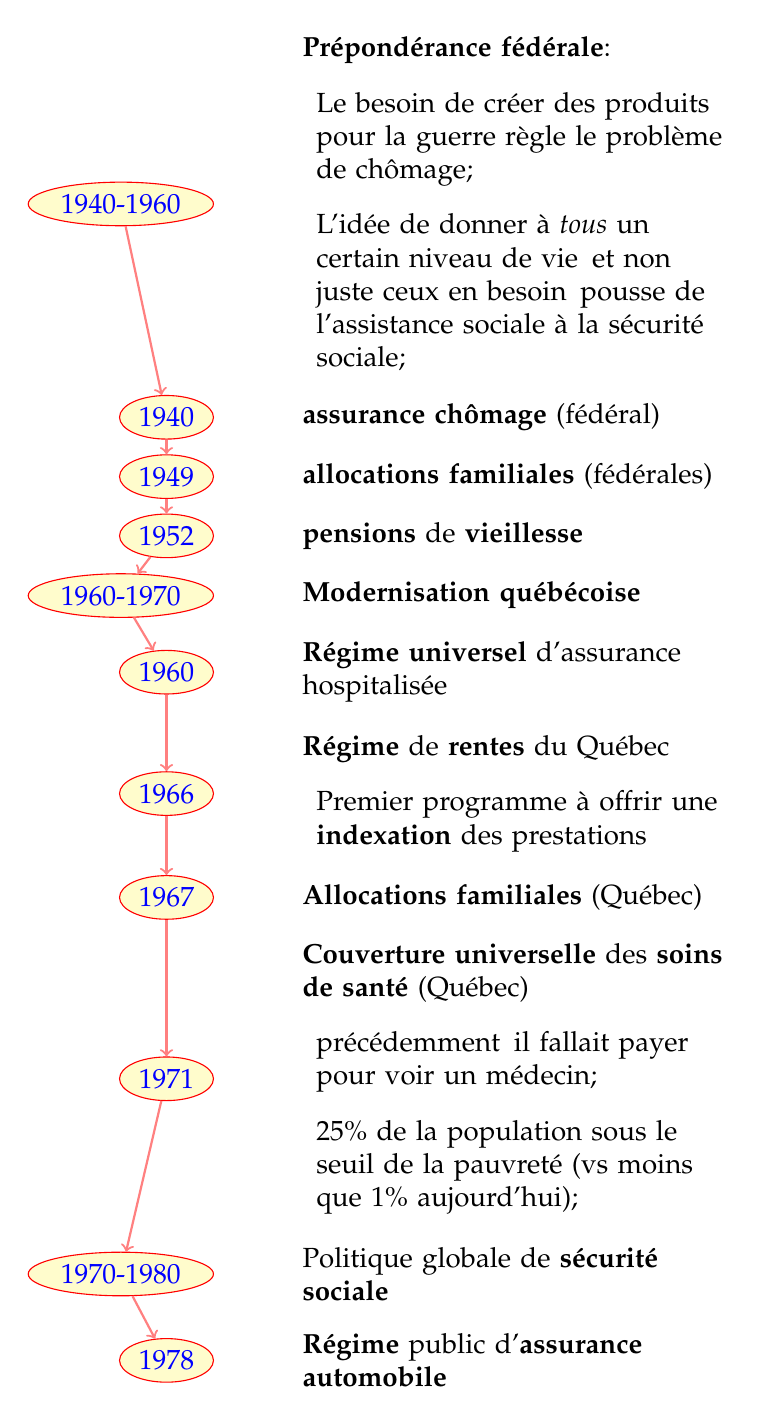
\begin{tikzpicture}[yscale = 0.5,%
           year/.style = {draw	= red,%
           				 text 	= blue,%
           				 fill 	= yellow!20,%
           				 shape 	= ellipse,%
           				 inner sep = 2pt%
           				 },%
           description/.style = {rectangle,%
           				 		align		= left,%
           				 		text width	= 55mm,%
           				 		anchor		= west%
           				 		},%
           timeline/.style = {->,%
           				 	 thick,%
           				 	 red!50%
           				 	 }%
           			]
    \foreach \year/\desc [count=\y] in {%
		1940-1960	/\textbf{Prépondérance fédérale}: 
		\begin{itemize}[leftmargin = *]
			\item	Le besoin de créer des produits pour la guerre règle le problème de chômage;
			\item	L'idée de donner à \textit{tous} un certain niveau de vie\, et non juste ceux en besoin\, pousse de l'assistance sociale à la sécurité sociale;
		\end{itemize},%
			1940	/	 \textbf{assurance chômage} (fédéral),%
			1949	/	 \textbf{allocations familiales} (fédérales),%
			1952	/	 \textbf{pensions} de \textbf{vieillesse},%
%%%	-----
%%%	NOTE:
%%%	+	fédéral ou provincial? (AJVR)
%%%
%%%	-----
       	1960-1970	/	\textbf{Modernisation québécoise},%
			1960	/	\textbf{Régime universel} d'assurance hospitalisée ,%
			1966	/	\textbf{Régime} de \textbf{rentes} du Québec
				\begin{itemize}[leftmargin = *]
				\item	Premier programme à offrir une \textbf{indexation} des prestations
				\end{itemize},%
			1967	/	 \textbf{Allocations familiales} (Québec),%
			1971	/	 \textbf{Couverture} \textbf{universelle} des \textbf{soins de santé} (Québec)
				\begin{itemize}[leftmargin = *]
				\item	précédemment\, il fallait payer pour voir un médecin;
				\item	25\% de la population sous le seuil de la pauvreté (vs moins que 1\% aujourd'hui);
				\end{itemize},%
       	1970-1980	/	Politique globale de \textbf{sécurité sociale},%
			1978	/	\textbf{Régime} public d'\textbf{assurance automobile} %
       } { \ifnum\y=1 \node[description](\y){\desc};
           \else\node[description,below=1ex of \z](\y){\desc};
           \fi
           \node[year](y-\y) [left=of \y] {\year};
           \ifnum\y>1\draw[timeline] (y-\z)-- (y-\y);\fi
           \global\let\z=\y% for drawing from last node
       }
\end{tikzpicture}

\textbf{Suite}:
\begin{itemize}
	\item	Poussée inflationniste, récession \textbf{(1981-1983)}, taux de chômage élevé;
	\item	Hausse des déficits et baisse des revenus fiscaux;
	\item	Recul de la protection sociale avec des programmes jugés extravagants;
	\item	Politiques de restriction budgétaire;
	\item	Explosion des coûts de l'assurance maladie
		\begin{itemize}
		\item[1984: ]	Loi canadienne sur la santé---pour préserver l'universalité des soins de santé;
		\end{itemize}
	\item	Coûts d'aucun \og bon sens \fg{} avec un régime qui \textbf{va} devoir changer;
		\begin{itemize}
		\item[1997:]	Assurance médicaments (Québec);
		\item[2006:]	Création d'assurance parentale (Québec);
		\end{itemize}
\end{itemize}

%%%%%%

\begin{conceptgen}{Programmes sociaux au Québec / Canada}
Les 9 fonctions de l'OIT sont couvert par ces programmes:
\begin{itemize}
	\item	Assurance sociale;
	\item	Assurance emploi;
	\item	Allocations familiales;
	\item	Indemnisation accidents travail (CEESST);
	\item	Régime de Rentes du Québec (RRQ);
	\item	Régime de Pension du Canada (RPC);
	\item	Pension sécurité vieillesse (fédéral) \textbf{\textit{ET}}\\ supplément de revenu garanti \textbf{\textit{ET}}\\ allocation au conjoint;
	\item	Régime de santé (maladie \textbf{\textit{ET}} hospitalisation---conjoint Canada-Québec);
	\item	Parentale;
	\item	Médicaments (Québec)
\end{itemize}
\end{conceptgen}

Catégories de programmes

\begin{tabularx}{\columnwidth}{| >{\columncolor{airforceblue!80}}>{\setlength\hsize{.25cm}} l | >{\columncolor{beaublue}}X  | >{\columncolor{beaublue}}X	|  >{\columncolor{beaublue}}X  |}
\hline\rowcolor{airforceblue} 
\textcolor{white}{\textbf{Programme}}	&	\textcolor{white}{\textbf{Assistance sociale}}	&	\textcolor{white}{\textbf{Assurance sociale}}		&	\textcolor{white}{\textbf{Régimes universels}}	\\\specialrule{0.1em}{0em}{0em} 
Objectif	&	protection minimale (dernier recourt)	&	protection de base			\\\hline
\end{tabularx}

\textbf{Assistance sociale}
\begin{itemize}[leftmargin = *]
	\item	Test de résidence;
	\item	Test de besoin;
	\item	Financement gouvernementale (Pay As You Go);
	\item	Aucune capitalisation (Pay As You Go);
%%%	-----
%%%	Comment trouves-tu ce format pour les commentaires? Je trouve ça pourrait être idéal!
%%%	NOTES: (AJVR)
%%%	+	je n'ai pas compris ce qu'elle voulait dire par pay as you go (AJVR);
%%%	+	Reste du stock à ajouter mais j'étais tanné un peu;
%%%		aide sociale au QC, 3 programmes
%%%	NOTES: (OC)
%%%	+	
%%%	-----
\end{itemize}

\textbf{Assurance sociale}
\begin{itemize}[leftmargin = *]
	\item	Contributions;
	\item	Programmes obligatoire;
	\item	Prestations en fonction de la participation et relié au gains;
	\item	Supervision gouvernementale;
	\item	Capitalisation totale ou partielle;
		\begin{itemize}
		\item	L'idée de la capitalisation est que c'est de l'argent mis de côté et pas inclus dans les revenus puisqu'elle sera éventuellement dépensée comme revenu.
		\end{itemize}
%%%	-----
%%%	NOTES (AJVR):
%%%	+	Développer sur contributions? 
%%%	+	Donner des exemples de programmes obligatoires;
%%%	+	Les prestations ça m'est un peu flou live j'ai moyen compris la façon qu'elle l'a dit mais j'en n'ai pas saise une assez bonne compréhension pour bien l'expliquer, toi?
%%%	-----
\begin{center}
\begin{tabular}{| >{\columncolor{beaublue}}c | >{\columncolor{beaublue}}c  |}
\hline\rowcolor{airforceblue} 
\textcolor{white}{\textbf{Avantages}}	&	\textcolor{white}{\textbf{Désavantages}}		\\\specialrule{0.1em}{0em}{0em} 
Protection de base	&	non-universel	\\\hline
Redistribution de l'argent	&	insuffisant	\\\hline
\end{tabular}
\end{center}
%%%	-----
%%%	Comment trouves-tu ce format pour les commentaires? Je trouve ça pourrait être idéal!
%%%	NOTES (AJVR):
%%%	+	Reste à développer sur ceci, voudrait peut-être la peine de ne pas le mettre en forme de tableau mais je me pratiquais;
%%%	+	Ajouter similitude avec assurance privée?
%%%	-----
\end{itemize}
%%%	-----
%%%	Breakdown de tableaux (AJVR):
%%%	Les tableaux c'est compliqué en LaTeX, je t'explique divers composantes ici:
%%%	+	Le premier argument après "begin{tabular}" est l'alignement des colonnes;
%%%	+	"c" pour center, "l" pour left-aligned, "r" pour right-aligned;
%%%	+	les barres "|" ajoute une barre verticale entre colonnes;
%%%	+	on met autant de lettre d'alignement que de colonnes désirées;
%%%	+	"tabular" est l'environnement pour créer les tables;
%%%	+	"airforceblue" est une des couleurs que j'ai défini dans le préambule, airforceblue!80 implique que j'y donne une opacité de 80%;
%%%	+	\columncolor va ensuite appliquer cette couleur à la _colonne_ en entier;
%%%	+	il est entouré de >{} pour y dire d'appliquer cette couleur à la position d'alignement "c"
%%%	+	en revanche, \rowcolor applique une couleur à une _rangée_ en entière;
%%%	+	\hline crée une _ligne_ _h_orizontale;
%%%	+	On sépare les items de la table avec "&" et fini la ligne avec "\\";
%%%	+	\shortstack crée comme une "boite" de texte ce qui fait que je peux créer plusieurs lignes;
%%%	+	Ceci sert uniquement à avoir plusieurs lignes de texte dans une même cellule;
%%%	+	\shortstack[l] est pour y indiquer d'aligner le texte à la gauche.
%%%	-----
\begin{center}
	\textbf{Comparaison d'assurance sociale et privée}
\begin{tabular}{| >{\columncolor{airforceblue!80}}l | >{\columncolor{beaublue}}l  | >{\columncolor{beaublue}}l |}
\hline\rowcolor{airforceblue} 
\textcolor{white}{\textbf{Assurance}}		&	\textcolor{white}{\textbf{Sociale}}		&	\textcolor{white}{\textbf{Privée}}		\\\specialrule{0.1em}{0em}{0em} 
Participation	&	obligatoire	&	facultative		\\\hline
Équité			&	sociale		&	individuelle		\\\hline
Base				&	légale		&	contractuelle	\\\hline
Contexte			&	monopole		&	compétition		\\\hline
\shortstack[l]{Facilité de \\ prévision des\\ coûts}	&	difficile 	&	\shortstack[l]{facile (tout\\ le monde\\ est couvert)}		\\\hline
Capitalisation	&	pas toujours	&	pleinement		\\\hline
\shortstack[l]{Sélection\\ des risques}	&	\shortstack[l]{aucune (peut pas \\ décider d'exclure\\ une personne)}	&	\\\hline
Indexation	&	au coût de la vie	&	rarement		\\\hline
But		&	sécurité sociale	&	\shortstack{couvrir ceux\\ qui le désirent}	\\\hline
\end{tabular}
\end{center}
Donc il y a des similitudes mais leur objectif diffère de façon significative.

\textbf{Régimes universels}
\begin{itemize}[leftmargin = *]
	\item	Obligatoire et universel;
	\item	Pas de tests de besoins;
	\item	Égalité basée sur la citoyenneté---tests de résidence;
	\item	Prestations fixes;
	\item	Pas de capitalisation (Pay As You Go);
%%%	-----
%%%	NOTES: (AJVR)
%%%	+	J'étais tanné et je n'ai vraiment pas mis beaucoup de détails rendu ici;
%%%	+	Ajouter
%%%	-----
\begin{center}
\begin{tabular}{| >{\columncolor{beaublue}}c | >{\columncolor{beaublue}}c  |}
\hline\rowcolor{airforceblue} 
\textcolor{white}{\textbf{Avantages}}	&	\textcolor{white}{\textbf{Désavantages}}		\\\specialrule{0.1em}{0em}{0em} 
Simple	&	Pas relié aux besoins	\\\hline
Combat la pauvreté	&	Coût caché	\\\hline
	&	Faibles prestations	\\\hline
\end{tabular}
\end{center}
\end{itemize}

Classement des régimes existants

%%%	-----
%%%	NOTES (AJVR):
%%%	+	Ce tableau est à retravailler dans un autre format je crois afin d'ajouter plus de détails d'Isabelle si t'en as, sinon c'est chill je vais faire du reformatting;
%%%	-----
\begin{tabular}{| >{\columncolor{beaublue}}m{3cm} | >{\columncolor{beaublue}}m{3cm} | >{\columncolor{beaublue}}m{3cm} |}
\hline\hline\rowcolor{airforceblue} 
\textcolor{white}{\textbf{Assurance emploi}}						&	\textcolor{white}{\textbf{Assistance sociale}}	&	\textcolor{white}{\textbf{Régimes universels}}	\\\hline
Assurance parentale					&	Assistance sociale						&	Allocations familiales	\\
Régime de rentes du Québec (R.R.Q.)	&	Prime au travail				&	soins de santé	\\
Santé Sécurité	au Travail (SST)		&	Supplément de revenu garanti	&	Sécurité de la vieillesse	\\
Assurance automobile					&	Allocation au conjoint					&	\\
Assurance médicament					&											&	\\\hline
\end{tabular}

\textbf{Régimes sociaux sous tension}

\textbf{Les États-Unis}


\end{multicols*}
\end{document}
